





\begin{frame}{Fundamentos de Criptografia}{}
\begin{itemize}
\pitem Quando fazemos compras pela internet, temos que enviar o número do cartão de crédito para efetivar a compra.
\item A internet é uma rede pública, e qualquer um pode acessar os pacotes de dados que são transmitidos através dela.
\pitem É mais seguro se você disfarçar os dados do seu cartão de alguma maneira.
\item E é o que fazemos quando, por exemplo, usamos um site que começa com ``https'' ao invés de ``http''.
\end{itemize}
\end{frame}


\begin{frame}{}{}
\begin{itemize}
\pitem Muitas informações podem ser roubadas em conexões pela internet.
\item Informações enviadas de/para forças armadas, diplomáticas,  cartão de crédito, etc...
\pitem Portanto além de precisarmos de formas de criptografar e decifrar informações, esse métodos precisam ser dificílimos de derrotar.
\end{itemize}
\end{frame}





\begin{frame}{O que é criptografia?}{}
\begin{itemize}
\pitem O estudo das técnicas de fazer comunicação segura entre duas partes,
onde existe uma terceira parte que não pode ter acesso à comunicação.

\pitem Imagine uma situação onde a pessoa A manda uma mensagem para a pessoa B,
mas somente a pessoa A e a pessoa B podem *entender* a mensagem,
apesar da imagem poder ser *acessada* por qualquer pessoa.

\end{itemize}
\end{frame}






\begin{frame}{}{}
\begin{tikzpicture}[shorten >=1pt,scale=0.6]%,on grid
\footnotesize
\tikzstyle{fantasma}=[minimum size=0cm]
\tikzstyle{bolota}=[shape=circle,thick,draw,minimum size=1.5cm]


\node[fantasma] at (0,0) (Alice) {Alice};
% \node[shape=rectangle,thick,draw] at (6,0) (encr) {$f(M)$};
% \node[shape=rectangle,thick,draw] at (12,0) (dese) {$g(C)$};
\node[fantasma] at (18,0) (Bob) {Bob};


\path[->,draw,thick] (Alice) edge node[fill=white, anchor=north, pos=0.5, align=center,yshift=-5pt] {$M$\\ Texto comum\\ (plain text)} (Bob);

% \path[->,draw,thick] (encr) edge node[fill=white, anchor=north, pos=0.5, align=center,yshift=-5pt] {$C$\\ Texto cifrado\\ (ciphertext)} (dese);

% \path[->,draw,thick] (dese) edge node[fill=white, anchor=north, pos=0.5, align=center,yshift=-5pt] {$M$} (Bob);


\visible<2->{\node[fantasma] at (9,4) (Mau) {Maurício};}
\node<2->[fantasma] at (9,0) (C) {};
\path<2->[->,draw,thick] (C) -- (Mau);

\end{tikzpicture}
\end{frame}





\begin{frame}{Exemplos}{}
\begin{itemize}

\pitem cartas enviadas que poderiam ser interceptadas sem correr o risco do interceptador conseguir ler o conteúdo. Júlio César, o imperador romano, tinha uma técnica de criptografia para que as cartas fossem enviadas de forma segura.
\pitem mensagens de rádio que podem ser ouvidas por terceiros, sem que estes terceiros entendam a mensagem. Alan Turing, cientista da computação, ficou famoso por fazer um computador capaz de **quebrar a criptografia** da inteligência nazista durante a segunda guerra mundial.

\end{itemize}
\end{frame}



\begin{frame}{}{}
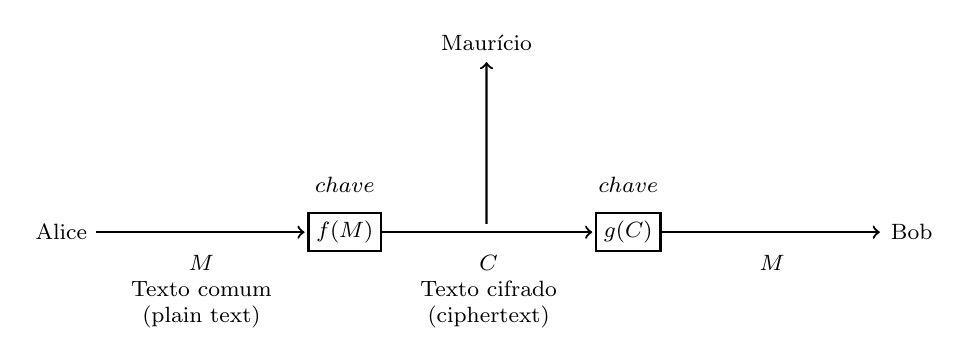
\begin{tikzpicture}[shorten >=1pt,scale=0.6]%,on grid
\footnotesize
\tikzstyle{fantasma}=[minimum size=0cm]
\tikzstyle{bolota}=[shape=circle,thick,draw,minimum size=1.5cm]


\node[fantasma] at (0,0) (Alice) {Alice};
\node[shape=rectangle,thick,draw] at (6,0) (encr) {$f(M)$};
\node[shape=rectangle,thick,draw] at (12,0) (dese) {$g(C)$};
\node[fantasma] at (18,0) (Bob) {Bob};


\path[->,draw,thick] (Alice) edge node[fill=white, anchor=north, pos=0.5, align=center,yshift=-5pt] {$M$\\ Texto comum\\ (plain text)} (encr);

\path[->,draw,thick] (encr) edge node[fill=white, anchor=north, pos=0.5, align=center,yshift=-5pt] {$C$\\ Texto cifrado\\ (ciphertext)} (dese);

\path[->,draw,thick] (dese) edge node[fill=white, anchor=north, pos=0.5, align=center,yshift=-5pt] {$M$} (Bob);


\visible<2->{\node[fantasma] at (9,4) (Mau) {Maurício};}
\node<2->[fantasma] at (9,0) (C) {};
\path<2->[->,draw,thick] (C) -- (Mau);

\node<3->[fantasma] at (6,1) (chave1) {$chave$};
\node<3->[fantasma] at (12,1) (chave1) {$chave$};
\end{tikzpicture}
\end{frame}



\begin{frame}{Cifra de deslocamento}{}
\begin{itemize}
\pitem Supostamente, Júlio César teria se comunicado com seus generais usando uma cifra de deslocamento.
\pitem Nessa cifra substitui-se cada letra pela que aparece 3 lugares adiante no alfabeto. \ppause

\begin{center}
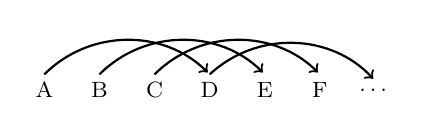
\begin{tikzpicture}[shorten >=1pt,scale=0.7]%,on grid
\footnotesize
\tikzstyle{fantasma}=[minimum size=0cm]
\tikzstyle{bolota}=[shape=circle,thick,draw,minimum size=1.5cm]


\node[fantasma] at (0,0) (A) {A};
\node[fantasma] at (1,0) (B) {B};
\node[fantasma] at (2,0) (C) {C};
\node[fantasma] at (3,0) (D) {D};
\node[fantasma] at (4,0) (E) {E};
\node[fantasma] at (5,0) (F) {F};
\node[fantasma] at (6,0) (etc) {\ldots};


\draw[->,thick] (A.north) to [bend left=45] (D.north);
\draw[->,thick] (B.north) to [bend left=45] (E.north);
\draw[->,thick] (C.north) to [bend left=45] (F.north);
\draw[->,thick] (D.north) to [bend left=45] (etc.north);
\end{tikzpicture}
\end{center}
\pitem Nesse caso a $chave$ é 3 o que é muito óbvio, então se quisermos usar a cifra de deslocamento, o ideal seria escolher outra chave. 
\end{itemize}
\end{frame}


\begin{frame}{}{}
\begin{center}
mnocaj ijikxvkj\ppause
\end{center}
\begin{columns}[t]\small
\begin{column}{0.33\textwidth}
0: mnocaj ijikxvkj\\\ppause
1: lmnb izhihjwuji\\
2: klmazhyghgivtih\\
3: jkl ygxfgfhushg\\\ppause
4: ijkzxfwefegtrgf\\
5: hijywevdedfsqfe\\
6: ghixvducdcerped\\
7: fghwuctbcbdqodc\\
8: efgvtbsabacpncb\\
\only<4>{9: defusar a bomba\\}
\only<5->{\bf \small 9: defusar a bomba\\}
\end{column}
\begin{column}{0.33\textwidth}
10: cdetr qz zanla \\
11: bcdsqzpyzy mk z\\
12: abcrpyoxyxzljzy\\
13:  abqoxnwxwykiyx\\
14: z apnwmvwvxjhxw\\
15: yz omvluvuwigwv\\
16: xyznluktutvhfvu\\
17: wxymktjstsugeut\\
18: vwxljsirsrtfdts\\
\end{column}
\begin{column}{0.33\textwidth}
19: uvwkirhqrqsecsr\\
20: tuvjhqgpqprdbrq\\
21: stuigpfopoqcaqp\\
22: rsthfoenonpb po\\
23: qrsgendmnmoazon\\
24: pqrfdmclmln ynm\\
25: opqeclbklkmzxml\\
26: nopdbkajkjlywlk\\\ppause
\end{column}
\end{columns}
\begin{center}
\ppause
defusar a bomba
\end{center}
\end{frame}



\begin{frame}{Cifra de substituição simples}{}
\begin{itemize}
\pitem Na cifra de deslocamento existem 26 chaves distintas, fácil de testar todas.
\pitem Mas podemos fazer algo mais seguro substituindo cada carácter por outro qualquer, não necessariamente o que está a 3 posições no alfabeto.
\end{itemize}
\ppause 

\ \\

{\footnotesize
\begin{tabular}{|p{0.14cm}|p{0.14cm}|p{0.14cm}|p{0.14cm}|p{0.14cm}|p{0.14cm}|p{0.14cm}|p{0.14cm}|p{0.14cm}|p{0.14cm}|p{0.14cm}|p{0.14cm}|p{0.14cm}|p{0.14cm}|p{0.14cm}|p{0.14cm}|p{0.14cm}|p{0.14cm}|p{0.14cm}|p{0.14cm}|p{0.14cm}|p{0.14cm}|p{0.14cm}|p{0.14cm}|p{0.14cm}|p{0.14cm}|}
\hline
a & b & c & d & e & f & g & h & i & j & k & l & m & n & o & p & q & r & s & t & u & v & w & x & y & z \\\hline
\end{tabular}

\begin{tabular}{|p{0.14cm}|p{0.14cm}|p{0.14cm}|p{0.14cm}|p{0.14cm}|p{0.14cm}|p{0.14cm}|p{0.14cm}|p{0.14cm}|p{0.14cm}|p{0.14cm}|p{0.14cm}|p{0.14cm}|p{0.14cm}|p{0.14cm}|p{0.14cm}|p{0.14cm}|p{0.14cm}|p{0.14cm}|p{0.14cm}|p{0.14cm}|p{0.14cm}|p{0.14cm}|p{0.14cm}|p{0.14cm}|p{0.14cm}|}
\hline
u & w & l & x & q & f & p & r & e & n & v & h & z & t & j & s & c & g & i & a & k & o & d & m & y & b \\\hline
\end{tabular}}
\end{frame}



\begin{frame}{}{}
\begin{itemize}
\pitem Agora existem $26!$ permutações (chaves) diferente, difícil de testar uma a uma.
\pitem Entretanto ainda é bastante fácil descobrir um texto criptografado dessa maneira.
\end{itemize}
\end{frame}



\begin{frame}{}{}
\small
\begin{columns}
\begin{column}{0.8\textwidth}
\texttt{j wjzwugxqej gkiij fje j sgezqegj pgutxq uauckq qz veqo xqixq j fetuh xq uwgeh tui khaezui iqzutui u gkiieu ljtlqtagjk iku jfqtieou sgetlesuhzqtaq tui hetrui xq fgqtaq tj hqiaq q tj ikh qzwjgu zjiljk jluiejtuhzqtaq uauckq jkagji hkpugqi tu luzsutru sugu xqiagkeg u etfguqiagkakgu zeheaug xu klguteu q whjckqug gqzqiiui xq ugzui jlexqtauei}
\begin{itemize}
\pitem Uma ideia é usar frequência de cada carácter, se soubermos que o texto está em português.
\end{itemize}
\end{column}
\begin{column}{0.2\textwidth}
\begin{tabular}{l|r}
u	& 41\\
q	& 33\\
i	& 26\\
g	& 24\\
j	& 22\\
e	& 21\\
t	& 21
\end{tabular}

Em pt-br.
\begin{tabular}{l|r}
  a & 	14.63\%\\
  e	& 12.57\%\\
  o	& 10.73\%\\
  s	& 7.81\%\\
  r	& 6.53\%\\
  i	& 6.18\%\\
  n	& 5.05\%
\end{tabular}
\end{column}
\end{columns}
\end{frame}


\begin{frame}{}{}
\small
\begin{columns}
\begin{column}{0.8\textwidth}
\begin{itemize}
\item u deve ser A.
\end{itemize}
\texttt{j wjzwAgxqej gkiij fje j sgezqegj pgAtxq AaAckq qz veqo xqixq j fetAh xq Awgeh tAi khaezAi iqzAtAi A gkiieA ljtlqtagjk ikA jfqtieoA sgetlesAhzqtaq tAi hetrAi xq fgqtaq tj hqiaq q tj ikh qzwjgA zjiljk jlAiejtAhzqtaq AaAckq jkagji hkpAgqi tA lAzsAtrA sAgA xqiagkeg A etfgAqiagkakgA zeheaAg xA klgAteA q whjckqAg gqzqiiAi xq AgzAi jlexqtaAei}
\begin{itemize}
\item Parece ok.
\end{itemize}
\end{column}
\begin{column}{0.2\textwidth}
\begin{tabular}{l|r}
u	& 41\\
q	& 33\\
i	& 26\\
g	& 24\\
j	& 22\\
e	& 21\\
t	& 21
\end{tabular}

Em pt-br.
\begin{tabular}{l|r}
  a & 	14.63\%\\
  e	& 12.57\%\\
  o	& 10.73\%\\
  s	& 7.81\%\\
  r	& 6.53\%\\
  i	& 6.18\%\\
  n	& 5.05\%
\end{tabular}
\end{column}
\end{columns}
\end{frame}


\begin{frame}{}{}
\small
\begin{columns}
\begin{column}{0.8\textwidth}
\begin{itemize}
\item q deve ser E.
\end{itemize}
\texttt{j wjzwAgxEej gkiij fje j sgezEegj pgAtxE AaAckE Ez veEo xEixE j fetAh xE Awgeh tAi khaezAi iEzAtAi A gkiieA ljtlEtagjk ikA jfEtieoA sgetlesAhzEtaE tAi hetrAi xE fgEtaE tj hEiaE E tj ikh EzwjgA zjiljk jlAiejtAhzEtaE AaAckE jkagji hkpAgEi tA lAzsAtrA sAgA xEiagkeg A etfgAEiagkakgA zeheaAg xA klgAteA E whjckEAg gEzEiiAi xE AgzAi jlexEtaAei}
\begin{itemize}
\item Parece ok.
\end{itemize}
\end{column}
\begin{column}{0.2\textwidth}
\begin{tabular}{l|r}
u	& 41\\
q	& 33\\
i	& 26\\
g	& 24\\
j	& 22\\
e	& 21\\
t	& 21
\end{tabular}

Em pt-br.
\begin{tabular}{l|r}
  a & 	14.63\%\\
  e	& 12.57\%\\
  o	& 10.73\%\\
  s	& 7.81\%\\
  r	& 6.53\%\\
  i	& 6.18\%\\
  n	& 5.05\%
\end{tabular}
\end{column}
\end{columns}
\end{frame}

\begin{frame}{}{}
\small
\begin{columns}
\begin{column}{0.8\textwidth}
\begin{itemize}
\item i deve ser O.
\end{itemize}
\texttt{j wjzwAgxEej gkOOj fje j sgezEegj pgAtxE AaAckE Ez veEo xEOxE j fetAh xE Awgeh tAO khaezAO OEzAtAO A gkOOeA ljtlEtagjk OkA jfEtOeoA sgetlesAhzEtaE tAO hetrAO xE fgEtaE tj hEOaE E tj Okh EzwjgA zjOljk jlAOejtAhzEtaE AaAckE jkagjO hkpAgEO tA lAzsAtrA sAgA xEOagkeg A etfgAEOagkakgA zeheaAg xA klgAteA E whjckEAg gEzEOOAO xE AgzAO jlexEtaAeO}
\begin{itemize}
\item Ficou estranho, note o OOAO. Pode ser S
\end{itemize}
\end{column}
\begin{column}{0.2\textwidth}
\begin{tabular}{l|r}
u	& 41\\
q	& 33\\
i	& 26\\
g	& 24\\
j	& 22\\
e	& 21\\
t	& 21
\end{tabular}

Em pt-br.
\begin{tabular}{l|r}
  a & 	14.63\%\\
  e	& 12.57\%\\
  o	& 10.73\%\\
  s	& 7.81\%\\
  r	& 6.53\%\\
  i	& 6.18\%\\
  n	& 5.05\%
\end{tabular}
\end{column}
\end{columns}
\end{frame}


\begin{frame}{}{}
\small
\begin{columns}
\begin{column}{0.8\textwidth}
\begin{itemize}
\item (i)O deve ser S.
\end{itemize}
\texttt{j wjzwAgxEej gkSSj fje j sgezEegj pgAtxE AaAckE Ez veEo xESxE j fetAh xE Awgeh tAS khaezAS SEzAtAS A gkSSeA ljtlEtagjk SkA jfEtSeoA sgetlesAhzEtaE tAS hetrAS xE fgEtaE tj hESaE E tj Skh EzwjgA zjSljk jlASejtAhzEtaE AaAckE jkagjS hkpAgES tA lAzsAtrA sAgA xESagkeg A etfgAESagkakgA zeheaAg xA klgAteA E whjckEAg gEzESSAS xE AgzAS jlexEtaAeS}
\begin{itemize}
\item Parece Ok.
\end{itemize}
\end{column}
\begin{column}{0.2\textwidth}
\begin{tabular}{l|r}
u	& 41\\
q	& 33\\
i	& 26\\
g	& 24\\
j	& 22\\
e	& 21\\
t	& 21
\end{tabular}

Em pt-br.
\begin{tabular}{l|r}
  a & 	14.63\%\\
  e	& 12.57\%\\
  o	& 10.73\%\\
  s	& 7.81\%\\
  r	& 6.53\%\\
  i	& 6.18\%\\
  n	& 5.05\%
\end{tabular}
\end{column}
\end{columns}
\end{frame}


\begin{frame}{}{}
\small
\begin{columns}
\begin{column}{0.8\textwidth}
\begin{itemize}
\item g deve ser O.
\end{itemize}
\texttt{j wjzwAOxEej OkSSj fje j sOezEeOj pOAtxE AaAckE Ez veEo xESxE j fetAh xE AwOeh tAS khaezAS SEzAtAS A OkSSeA ljtlEtaOjk SkA jfEtSeoA sOetlesAhzEtaE tAS hetrAS xE fOEtaE tj hESaE E tj Skh EzwjOA zjSljk jlASejtAhzEtaE AaAckE jkaOjS hkpAOES tA lAzsAtrA sAOA xESaOkeO A etfOAESaOkakOA zeheaAO xA klOAteA E whjckEAO OEzESSAS xE AOzAS jlexEtaAeS}
\begin{itemize}
\item Note a palavra OEzESSAS. Deve ser R
\end{itemize}
\end{column}
\begin{column}{0.2\textwidth}
\begin{tabular}{l|r}
u	& 41\\
q	& 33\\
i	& 26\\
g	& 24\\
j	& 22\\
e	& 21\\
t	& 21
\end{tabular}

Em pt-br.
\begin{tabular}{l|r}
  a & 	14.63\%\\
  e	& 12.57\%\\
  o	& 10.73\%\\
  s	& 7.81\%\\
  r	& 6.53\%\\
  i	& 6.18\%\\
  n	& 5.05\%
\end{tabular}
\end{column}
\end{columns}
\end{frame}



\begin{frame}{}{}
\small
\begin{columns}
\begin{column}{0.8\textwidth}
\begin{itemize}
\item (g)O deve ser R.
\end{itemize}
\texttt{j wjzwARxEej RkSSj fje j sRezEeRj pRAtxE AaAckE Ez veEo xESxE j fetAh xE AwReh tAS khaezAS SEzAtAS A RkSSeA ljtlEtaRjk SkA jfEtSeoA sRetlesAhzEtaE tAS hetrAS xE fREtaE tj hESaE E tj Skh EzwjRA zjSljk jlASejtAhzEtaE AaAckE jkaRjS hkpARES tA lAzsAtrA sARA xESaRkeR A etfRAESaRkakRA zeheaAR xA klRAteA E whjckEAR REzESSAS xE ARzAS jlexEtaAeS}
\begin{itemize}
\item Parece ok.
\end{itemize}
\end{column}
\begin{column}{0.2\textwidth}
\begin{tabular}{l|r}
u	& 41\\
q	& 33\\
i	& 26\\
g	& 24\\
j	& 22\\
e	& 21\\
t	& 21
\end{tabular}

Em pt-br.
\begin{tabular}{l|r}
  a & 	14.63\%\\
  e	& 12.57\%\\
  o	& 10.73\%\\
  s	& 7.81\%\\
  r	& 6.53\%\\
  i	& 6.18\%\\
  n	& 5.05\%
\end{tabular}
\end{column}
\end{columns}
\end{frame}



\begin{frame}{}{}
\small
\begin{columns}
\begin{column}{0.8\textwidth}
\begin{itemize}
\item j deve ser O.
\end{itemize}
\texttt{O wOzwARxEeO RkSSO fOe O sRezEeRO pRAtxE AaAckE Ez veEo xESxE O fetAh xE AwReh tAS khaezAS SEzAtAS A RkSSeA lOtlEtaROk SkA OfEtSeoA sRetlesAhzEtaE tAS hetrAS xE fREtaE tO hESaE E tO Skh EzwORA zOSlOk OlASeOtAhzEtaE AaAckE OkaROS hkpARES tA lAzsAtrA sARA xESaRkeR A etfRAESaRkakRA zeheaAR xA klRAteA E whOckEAR REzESSAS xE ARzAS OlexEtaAeS}
\begin{itemize}
\item Parece ok.
\end{itemize}
\end{column}
\begin{column}{0.2\textwidth}
\begin{tabular}{l|r}
u	& 41\\
q	& 33\\
i	& 26\\
g	& 24\\
j	& 22\\
e	& 21\\
t	& 21
\end{tabular}

Em pt-br.
\begin{tabular}{l|r}
  a & 	14.63\%\\
  e	& 12.57\%\\
  o	& 10.73\%\\
  s	& 7.81\%\\
  r	& 6.53\%\\
  i	& 6.18\%\\
  n	& 5.05\%

\end{tabular}
\end{column}
\end{columns}
\end{frame}


\begin{frame}{}{}
\small
\begin{columns}
\begin{column}{0.8\textwidth}
\begin{itemize}
\item e deve ser I.
\end{itemize}
\texttt{O wOzwARxEIO RkSSO fOI O sRIzEIRO pRAtxE AaAckE Ez vIEo xESxE O fItAh xE AwRIh tAS khaIzAS SEzAtAS A RkSSIA lOtlEtaROk SkA OfEtSIoA sRItlIsAhzEtaE tAS hItrAS xE fREtaE tO hESaE E tO Skh EzwORA zOSlOk OlASIOtAhzEtaE AaAckE OkaROS hkpARES tA lAzsAtrA sARA xESaRkIR A ItfRAESaRkakRA zIhIaAR xA klRAtIA E whOckEAR REzESSAS xE ARzAS OlIxEtaAIS}
\begin{itemize}
\item Parece ok.
\end{itemize}
\end{column}
\begin{column}{0.2\textwidth}
\begin{tabular}{l|r}
u	& 41\\
q	& 33\\
i	& 26\\
g	& 24\\
j	& 22\\
e	& 21\\
t	& 21
\end{tabular}

Em pt-br.
\begin{tabular}{l|r}
  a & 	14.63\%\\
  e	& 12.57\%\\
  o	& 10.73\%\\
  s	& 7.81\%\\
  r	& 6.53\%\\
  i	& 6.18\%\\
  n	& 5.05\%
\end{tabular}
\end{column}
\end{columns}
\end{frame}


\begin{frame}{}{}
\small
\begin{columns}
\begin{column}{0.8\textwidth}
\begin{itemize}
\item t deve ser N.
\end{itemize}
\texttt{O wOzwARxEIO RkSSO fOI O sRIzEIRO pRANxE AaAckE Ez vIEo xESxE O fINAh xE AwRIh NAS khaIzAS SEzANAS A RkSSIA lONlENaROk SkA OfENSIoA sRINlIsAhzENaE NAS hINrAS xE fRENaE NO hESaE E NO Skh EzwORA zOSlOk OlASIONAhzENaE AaAckE OkaROS hkpARES NA lAzsANrA sARA xESaRkIR A INfRAESaRkakRA zIhIaAR xA klRANIA E whOckEAR REzESSAS xE ARzAS OlIxENaAIS}
\begin{itemize}
\item Parece ok.
\end{itemize}
\end{column}
\begin{column}{0.2\textwidth}
\begin{tabular}{l|r}
u	& 41\\
q	& 33\\
i	& 26\\
g	& 24\\
j	& 22\\
e	& 21\\
t	& 21
\end{tabular}

Em pt-br.
\begin{tabular}{l|r}
  a & 	14.63\%\\
  e	& 12.57\%\\
  o	& 10.73\%\\
  s	& 7.81\%\\
  r	& 6.53\%\\
  i	& 6.18\%\\
  n	& 5.05\%
\end{tabular}
\end{column}
\end{columns}
\end{frame}


\begin{frame}{}{}
\small
\begin{itemize}
\item O próximo seria k por D.
\end{itemize}
\texttt{O wOzwARxEIO RDSSO fOI O sRIzEIRO pRANxE AaAcDE Ez vIEo xESxE O fINAh xE AwRIh NAS DhaIzAS SEzANAS A RDSSIA lONlENaROD SDA OfENSIoA sRINlIsAhzENaE NAS hINrAS xE fRENaE NO hESaE E NO SDh EzwORA zOSlOD OlASIONAhzENaE AaAcDE ODaROS hDpARES NA lAzsANrA sARA xESaRDIR A INfRAESaRDaDRA zIhIaAR xA DlRANIA E whOcDEAR REzESSAS xE ARzAS OlIxENaAIS}
\begin{itemize}
\pitem Ficou estranho, olhe o "RDSSO". Deve ser U.
\pitem Daqui pra frente começa a falhar um pouco. 
\end{itemize}
\end{frame}

\begin{frame}{}{}
\small
\begin{itemize}
\item (k)D por U.
\end{itemize}
\texttt{O wOzwARxEIO RUSSO fOI O sRIzEIRO pRANxE AaAcUE Ez vIEo xESxE O fINAh xE AwRIh NAS UhaIzAS SEzANAS A RUSSIA lONlENaROU SUA OfENSIoA sRINlIsAhzENaE NAS hINrAS xE fRENaE NO hESaE E NO SUh EzwORA zOSlOU OlASIONAhzENaE AaAcUE OUaROS hUpARES NA lAzsANrA sARA xESaRUIR A INfRAESaRUaURA zIhIaAR xA UlRANIA E whOcUEAR REzESSAS xE ARzAS OlIxENaAIS}
\begin{itemize}
\pitem REzESSAS deve ser REMESSAS.
\pitem Trocar z por M. 
\end{itemize}
\end{frame}

\begin{frame}{}{}
\small
\begin{itemize}
\item z por M.
\end{itemize}
\texttt{O wOMwARxEIO RUSSO fOI O sRIMEIRO pRANxE AaAcUE EM vIEo xESxE O fINAh xE AwRIh NAS UhaIMAS SEMANAS A RUSSIA lONlENaROU SUA OfENSIoA sRINlIsAhMENaE NAS hINrAS xE fRENaE NO hESaE E NO SUh EMwORA MOSlOU OlASIONAhMENaE AaAcUE OUaROS hUpARES NA lAMsANrA sARA xESaRUIR A INfRAESaRUaURA MIhIaAR xA UlRANIA E whOcUEAR REMESSAS xE ARMAS OlIxENaAIS}
\begin{itemize}
\pitem tem xE, xA..
\pitem x deve ser D
\end{itemize}
\end{frame}

\begin{frame}{}{}
\small
\begin{itemize}
\item x por D.
\end{itemize}
\texttt{O wOMwARDEIO RUSSO fOI O sRIMEIRO pRANDE AaAcUE EM vIEo DESDE O fINAh DE AwRIh NAS UhaIMAS SEMANAS A RUSSIA lONlENaROU SUA OfENSIoA sRINlIsAhMENaE NAS hINrAS DE fRENaE NO hESaE E NO SUh EMwORA MOSlOU OlASIONAhMENaE AaAcUE OUaROS hUpARES NA lAMsANrA sARA DESaRUIR A INfRAESaRUaURA MIhIaAR DA UlRANIA E whOcUEAR REMESSAS DE ARMAS OlIDENaAIS}
\begin{itemize}
\pitem sRIMEIRO deve ser PRIMEIRO
\pitem s deve ser P
\end{itemize}
\end{frame}

\begin{frame}{}{}
\small
\begin{itemize}
\item s por P.
\end{itemize}
\texttt{O wOMwARDEIO RUSSO fOI O PRIMEIRO pRANDE AaAcUE EM vIEo DESDE O fINAh DE AwRIh NAS UhaIMAS SEMANAS A RUSSIA lONlENaROU SUA OfENSIoA PRINlIPAhMENaE NAS hINrAS DE fRENaE NO hESaE E NO SUh EMwORA MOSlOU OlASIONAhMENaE AaAcUE OUaROS hUpARES NA lAMPANrA PARA DESaRUIR A INfRAESaRUaURA MIhIaAR DA UlRANIA E whOcUEAR REMESSAS DE ARMAS OlIDENaAIS}
\begin{itemize}
\pitem pRANDE deve ser GRANDE
\pitem p deve ser G
\end{itemize}
\end{frame}

\begin{frame}{}{}
\small
\begin{itemize}
\item p por G.
\end{itemize}
\texttt{O wOMwARDEIO RUSSO fOI O PRIMEIRO GRANDE AaAcUE EM vIEo DESDE O fINAh DE AwRIh NAS UhaIMAS SEMANAS A RUSSIA lONlENaROU SUA OfENSIoA PRINlIPAhMENaE NAS hINrAS DE fRENaE NO hESaE E NO SUh EMwORA MOSlOU OlASIONAhMENaE AaAcUE OUaROS hUGARES NA lAMPANrA PARA DESaRUIR A INfRAESaRUaURA MIhIaAR DA UlRANIA E whOcUEAR REMESSAS DE ARMAS OlIDENaAIS}
\begin{itemize}
\pitem hUGARES deve ser LUGARES
\pitem h deve ser L
\end{itemize}
\end{frame}

\begin{frame}{}{}
\small
\begin{itemize}
\item h por L.
\end{itemize}
\texttt{O wOMwARDEIO RUSSO fOI O PRIMEIRO GRANDE AaAcUE EM vIEo DESDE O fINAL DE AwRIL NAS ULaIMAS SEMANAS A RUSSIA lONlENaROU SUA OfENSIoA PRINlIPALMENaE NAS LINrAS DE fRENaE NO LESaE E NO SUL EMwORA MOSlOU OlASIONALMENaE AaAcUE OUaROS LUGARES NA lAMPANrA PARA DESaRUIR A INfRAESaRUaURA MILIaAR DA UlRANIA E wLOcUEAR REMESSAS DE ARMAS OlIDENaAIS}
\begin{itemize}
\pitem INfRAESaRUaURA deve ser INFRAESTRUTURA
\pitem f deve ser F mesmo, e a deve ser T
\end{itemize}
\end{frame}

\begin{frame}{}{}
\small
\begin{itemize}
\item  f por F, a por T
\end{itemize}
\texttt{O wOMwARDEIO RUSSO fOI O PRIMEIRO GRANDE ATAcUE EM vIEo DESDE O fINAL DE AwRIL NAS ULTIMAS SEMANAS A RUSSIA lONlENTROU SUA OfENSIoA PRINlIPALMENTE NAS LINrAS DE fRENTE NO LESTE E NO SUL EMwORA MOSlOU OlASIONALMENTE ATAcUE OUTROS LUGARES NA lAMPANrA PARA DESTRUIR A INfRAESTRUTURA MILITAR DA UlRANIA E wLOcUEAR REMESSAS DE ARMAS OlIDENTAIS}
\begin{itemize}
\pitem OlIDENTAIS deve ser OCIDENTAIS
\pitem l deve ser C. E assim por diante.
\end{itemize}
\end{frame}


\begin{frame}{}{}
\small
\begin{itemize}
\item  terminando
\end{itemize}
\texttt{O BOMBARDEIO RUSSO FOI O PRIMEIRO GRANDE ATAQUE EM KIEV DESDE O FINAL DE ABRIL NAS ULTIMAS SEMANAS A RUSSIA CONCENTROU SUA OFENSIVA PRINCIPALMENTE NAS LINHAS DE FRENTE NO LESTE E NO SUL EMBORA MOSCOU OCASIONALMENTE ATAQUE OUTROS LUGARES NA CAMPANHA PARA DESTRUIR A INFRAESTRUTURA MILITAR DA UCRANIA E BLOQUEAR REMESSAS DE ARMAS OCIDENTAIS}
\begin{itemize}
\pitem Note que não é preciso muito esforço.
\pitem Mesmo tendo 26! chaves.
\end{itemize}
\end{frame}


\begin{frame}{}{}
\begin{itemize}
\pitem Além disso, suponha que você vai encriptar o número do cartão de crédito trocando os dígitos de 0 a 9. 
\pitem Nesse caso seriam apenas 10! chaves possíveis, ou 3.628.800.
\pitem Que é possível simplesmente testar todas as combinações. Em particular se Maurício tiver roubado o número encriptado de vários cartões.
\end{itemize}
\end{frame}



\begin{frame}{Cifras de Chave Única}{}
\begin{itemize}
\pitem Uma criptografia mais robusta que a cifra de substituição simples. Envolve a utilização de uma chave maior, e da operação $\oplus$ (XOR, ou exclusivo).
\begin{align}
0 \oplus 0 &= 0 \\
0 \oplus 1 &= 1 \\
1 \oplus 0 &= 1 \\
1 \oplus 1 &= 0 
\end{align}
\end{itemize}
\end{frame}

\begin{frame}{}{}
\begin{itemize}
\pitem A cifra de chave única se baseia no fato de que se ao bit $x$ é aplicado um XOR com um bit $y$ duas vezes, ele volta a ser $x$, ou seja,
$$
(x \oplus y) \oplus y = x
$$

\pitem Você pode entender o XOR como: se $y$ for 0 o resultado é o $x$, se $y$ for 1 o resultado é o inverso de $x$.
\end{itemize}
\end{frame}


\begin{frame}{}{}
\begin{itemize}
\pitem Toda informação digital pode ser convertida em bits. Utilizando o padrão ASCII por exemplo:
\end{itemize}
\begin{center}
\begin{tabular}{ccccc}
& b & o & m & b \\
\ppause & 98 & 111 & 109 & 98 \\
\ppause $M$     & 0110 0010 & 0110 1111 & 0110 1101 & 0110 0010 \\
\ppause & $\oplus$ & $\oplus$ & $\oplus$ & $\oplus$ \\
        $chave$ & 0011 0101 & 0010 0000 & 1101 1111 & 0110 1011 \\
\ppause $C$     & 0101 0111 & 0100 1111 & 1011 0010 & 0000 1001
\end{tabular}
\end{center}
\end{frame}



\begin{frame}{}{}
\begin{center}
\begin{tabular}{ccccc}
& b & o & m & b \\
\ppause & 98 & 111 & 109 & 98 \\
\ppause $M$     & 0110 0010 & 0110 1111 & 0110 1101 & 0110 0010 \\
\ppause & $\oplus$ & $\oplus$ & $\oplus$ & $\oplus$ \\
        $chave$ & 0011 0101 & 0010 0000 & 1101 1111 & 0110 1011 \\
\ppause $C$     & 0101 0111 & 0100 1111 & 1011 0010 & 0000 1001 \\
\ppause & $\oplus$ & $\oplus$ & $\oplus$ & $\oplus$ \\
        $chave$ & 0011 0101 & 0010 0000 & 1101 1111 & 0110 1011 \\
\ppause $M$     & 0110 0010 & 0110 1111 & 0110 1101 & 0110 0010 \\
\ppause & b & o & m & b 
\end{tabular}
\end{center}
\end{frame}




\begin{frame}{}{}
\begin{itemize}
\pitem Se todos os bits da chave forem gerados aleatoriamente.
\pitem Cada bit de $C$ tem 50\% de chance de ser igual ao bit original e 50\% de ser o inverso.
\item Ou seja, o bit de $C$ não te dará nenhuma informação sobre $M$, ou sobre a chave.
\pitem Portanto podemos considerar que é uma criptografia robusta nesse sentido, entretanto...
\end{itemize}
\end{frame}



\begin{frame}{}{}
Desvantagens da cifra de chave única.
\begin{itemize}
\pitem Se $M$ exige $b$ bits, então a chave precisa ter $b$ bits.
\pitem Você só pode usar a chave uma única vez:
\begin{itemize}
\item Suponha que Maurício obtenha 2 textos cifrados $C_1$ e $C_2$.
\pitem Apesar de não ter a chave Maurício faz 
\begin{align}
C_1 &\oplus C_2 \\
(M_1 \oplus chave) & \oplus (M_2 \oplus chave) \\
M_1 & \oplus M_2 
\end{align}
\pitem Ou seja, Maurício obtém a informação dos bits em que as mensagens originais era iguais (inclusive se ela for toda igual)
\end{itemize}
\end{itemize}
\end{frame}



\begin{frame}{Cifra de bloco e encadeamento}{}
\begin{itemize}
\pitem Quanto a mensagem a ser passada é muito grande, precisar de uma chave igualmente grande pode ser ruim.
\pitem Podemos usar uma chave mais curta e desmembrar o $M$ em vários blocos, aplicando a chave em cada bloco.
\end{itemize}
\end{frame}

\begin{frame}{}{}
\begin{itemize}
\pitem Digamos que temos uma função $E()$ que usa uma certa $chave$ e consegue encriptar um bloco de tamanho $b$.
\pitem Quebramos nosso texto comum $M$ em blocos $t_1, t_2, \ldots, t_l$, cada um com tamanho $b$.
\pitem Poderíamos agora encriptar cada bloco com $E()$, porém isso ainda daria informação à Maurício sobre quais blocos de $M$ são iguais.
\pitem Então aplicamos a técnica de encadeamento.
\end{itemize}
\end{frame}




\begin{frame}{}{}
\begin{align}
c_1 & = E(t_1)\\
c_2 & = E(t_2 \oplus c_1)\\
c_3 & = E(t_3 \oplus c_2)\\
& \ldots \\
c_l & = E(t_l \oplus c_{l-1})
\end{align}
\ppause 
Maurício agora não consegue ver quais blocos são iguais, entretanto se a mensagem for toda igual, a sequencia de blocos também será. Vamos consertar isso com um {\bf vetor de inicialização} $c_0$ gerado aleatoriamente.
\end{frame}



\begin{frame}{}{}
\begin{align}
c_0 & = random();\\
c_1 & = E(t_1 \oplus c_0)\\
c_2 & = E(t_2 \oplus c_1)\\
c_3 & = E(t_3 \oplus c_2)\\
& \ldots \\
c_l & = E(t_l \oplus c_{l-1})
\end{align}
\end{frame}



\begin{frame}{}{}
\begin{itemize}
\pitem Bob por sua vez, tem a função $D$ e $chave$ capaz de decifrar um bloco de tamanho $b$ e recebe os blocos $c_0, c_1, c_2, \ldots, c_l$.
\end{itemize}
\begin{align}
t_1 &= D(c_1) \oplus c_0 = (t_1 \oplus c_0) \oplus c_0\\\ppause
t_2 &= D(c_2) \oplus c_1 \\
t_3 &= D(c_2) \oplus c_2 \\
& \ldots \\
t_l &= D(c_l) \oplus c_{l-1}
\end{align}
\end{frame}



\begin{frame}{}{}
\begin{itemize}
\pitem Um exemplo desse sistema é o AES ({\it Advanced Encryption Standard}) que faz algo mais elaborado que um XOR, e usa chaves de 128, 192 ou 256 bits para encriptar blocos de 128 bits.
\pitem Apesar de eficiente esses sistemas tem um grande desafio. Ambas as partes precisam concordar com a $chave$ a priori.
\pitem Seria ineficiente, que todo site que frequentamos/compramos exigisse que fossemos num lugar físico pegar a chave em um pendrive.
\end{itemize}
\end{frame}

